\section{子问题二：家庭充电设施安装潜力预测}

\subsection{问题定义与难点}

任务二的目标是预测home\_charging\_available（二分类：0/1），即识别具备家庭充电条件的用户。该任务在评分体系中权重最高（40\%），评估指标仅采用准确率。

模型从数据中学习的是当前家庭充电可用状态的标注模式。将预测为1的用户划入安装潜力较高人群，是对数据列原始语义的忠实映射，其产出可直接服务于充电设施推广决策。

\textbf{标签含义界定}是本任务的首要前提。赛题目标变量名称与数据描述之间存在语义差距："当前充电可用状态"反映既有设施条件，"安装潜力"则指向未来行为。两个概念的差异划定了建模框架的基本边界。\textbf{下游变量风险}需要关注。ev\_adoption\_likelihood很可能是家庭充电条件的下游结果（拥有家充条件的用户因此表现出较高的采用意愿），因果方向恰与预测任务相反。用下游标签预测上游条件属于逻辑上的反向因果，主方案排除该变量。\textbf{单变量区分度极低}。EDA中，有家充与无家充群体在最近充电站距离上中位数完全一致（6.9 km），三种城市类型的家充比例差异不超过0.4个百分点（64.8\%--65.2\%）。原始特征对目标无区分能力。

\subsection{探索性数据分析}

\subsubsection{目标变量分布}

家充可用用户占比65.0\%，类别呈轻度不平衡（图\ref{fig:t2_target}）。

\begin{figure}[H]
\centering
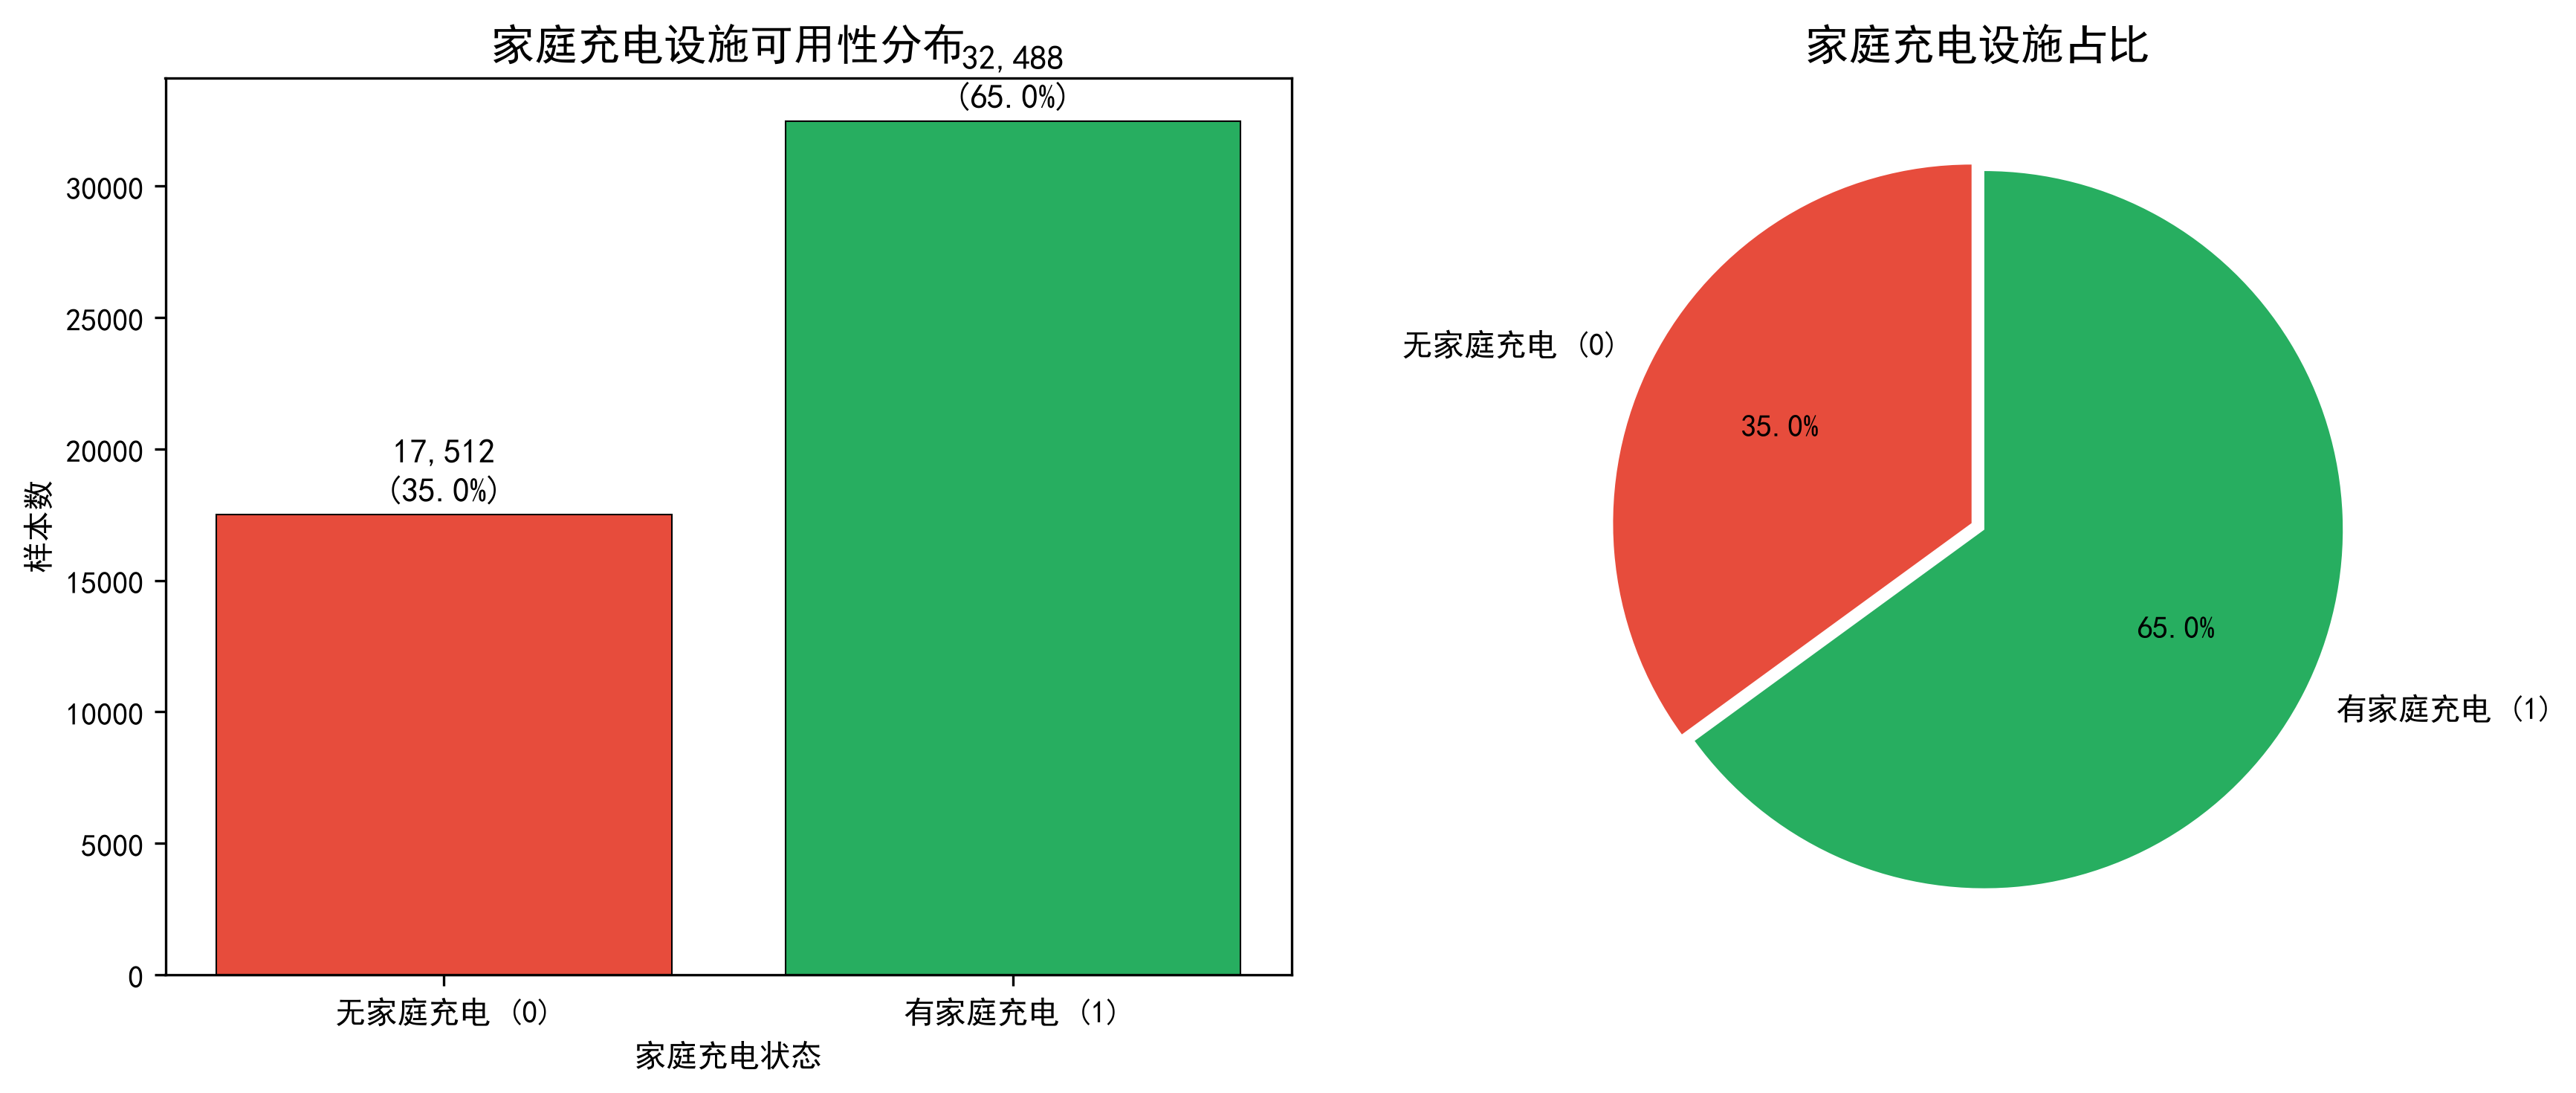
\includegraphics[width=0.85\textwidth]{figures/task2_target_distribution.png}
\caption{家庭充电设施可用性分布}
\label{fig:t2_target}
\end{figure}

\subsubsection{充电站距离与家充状态}

如图\ref{fig:t2_dist}所示，有/无家庭充电的群体在最近充电站距离上的中位数完全相同（6.9 km），单变量区分度为零。

\begin{figure}[H]
\centering
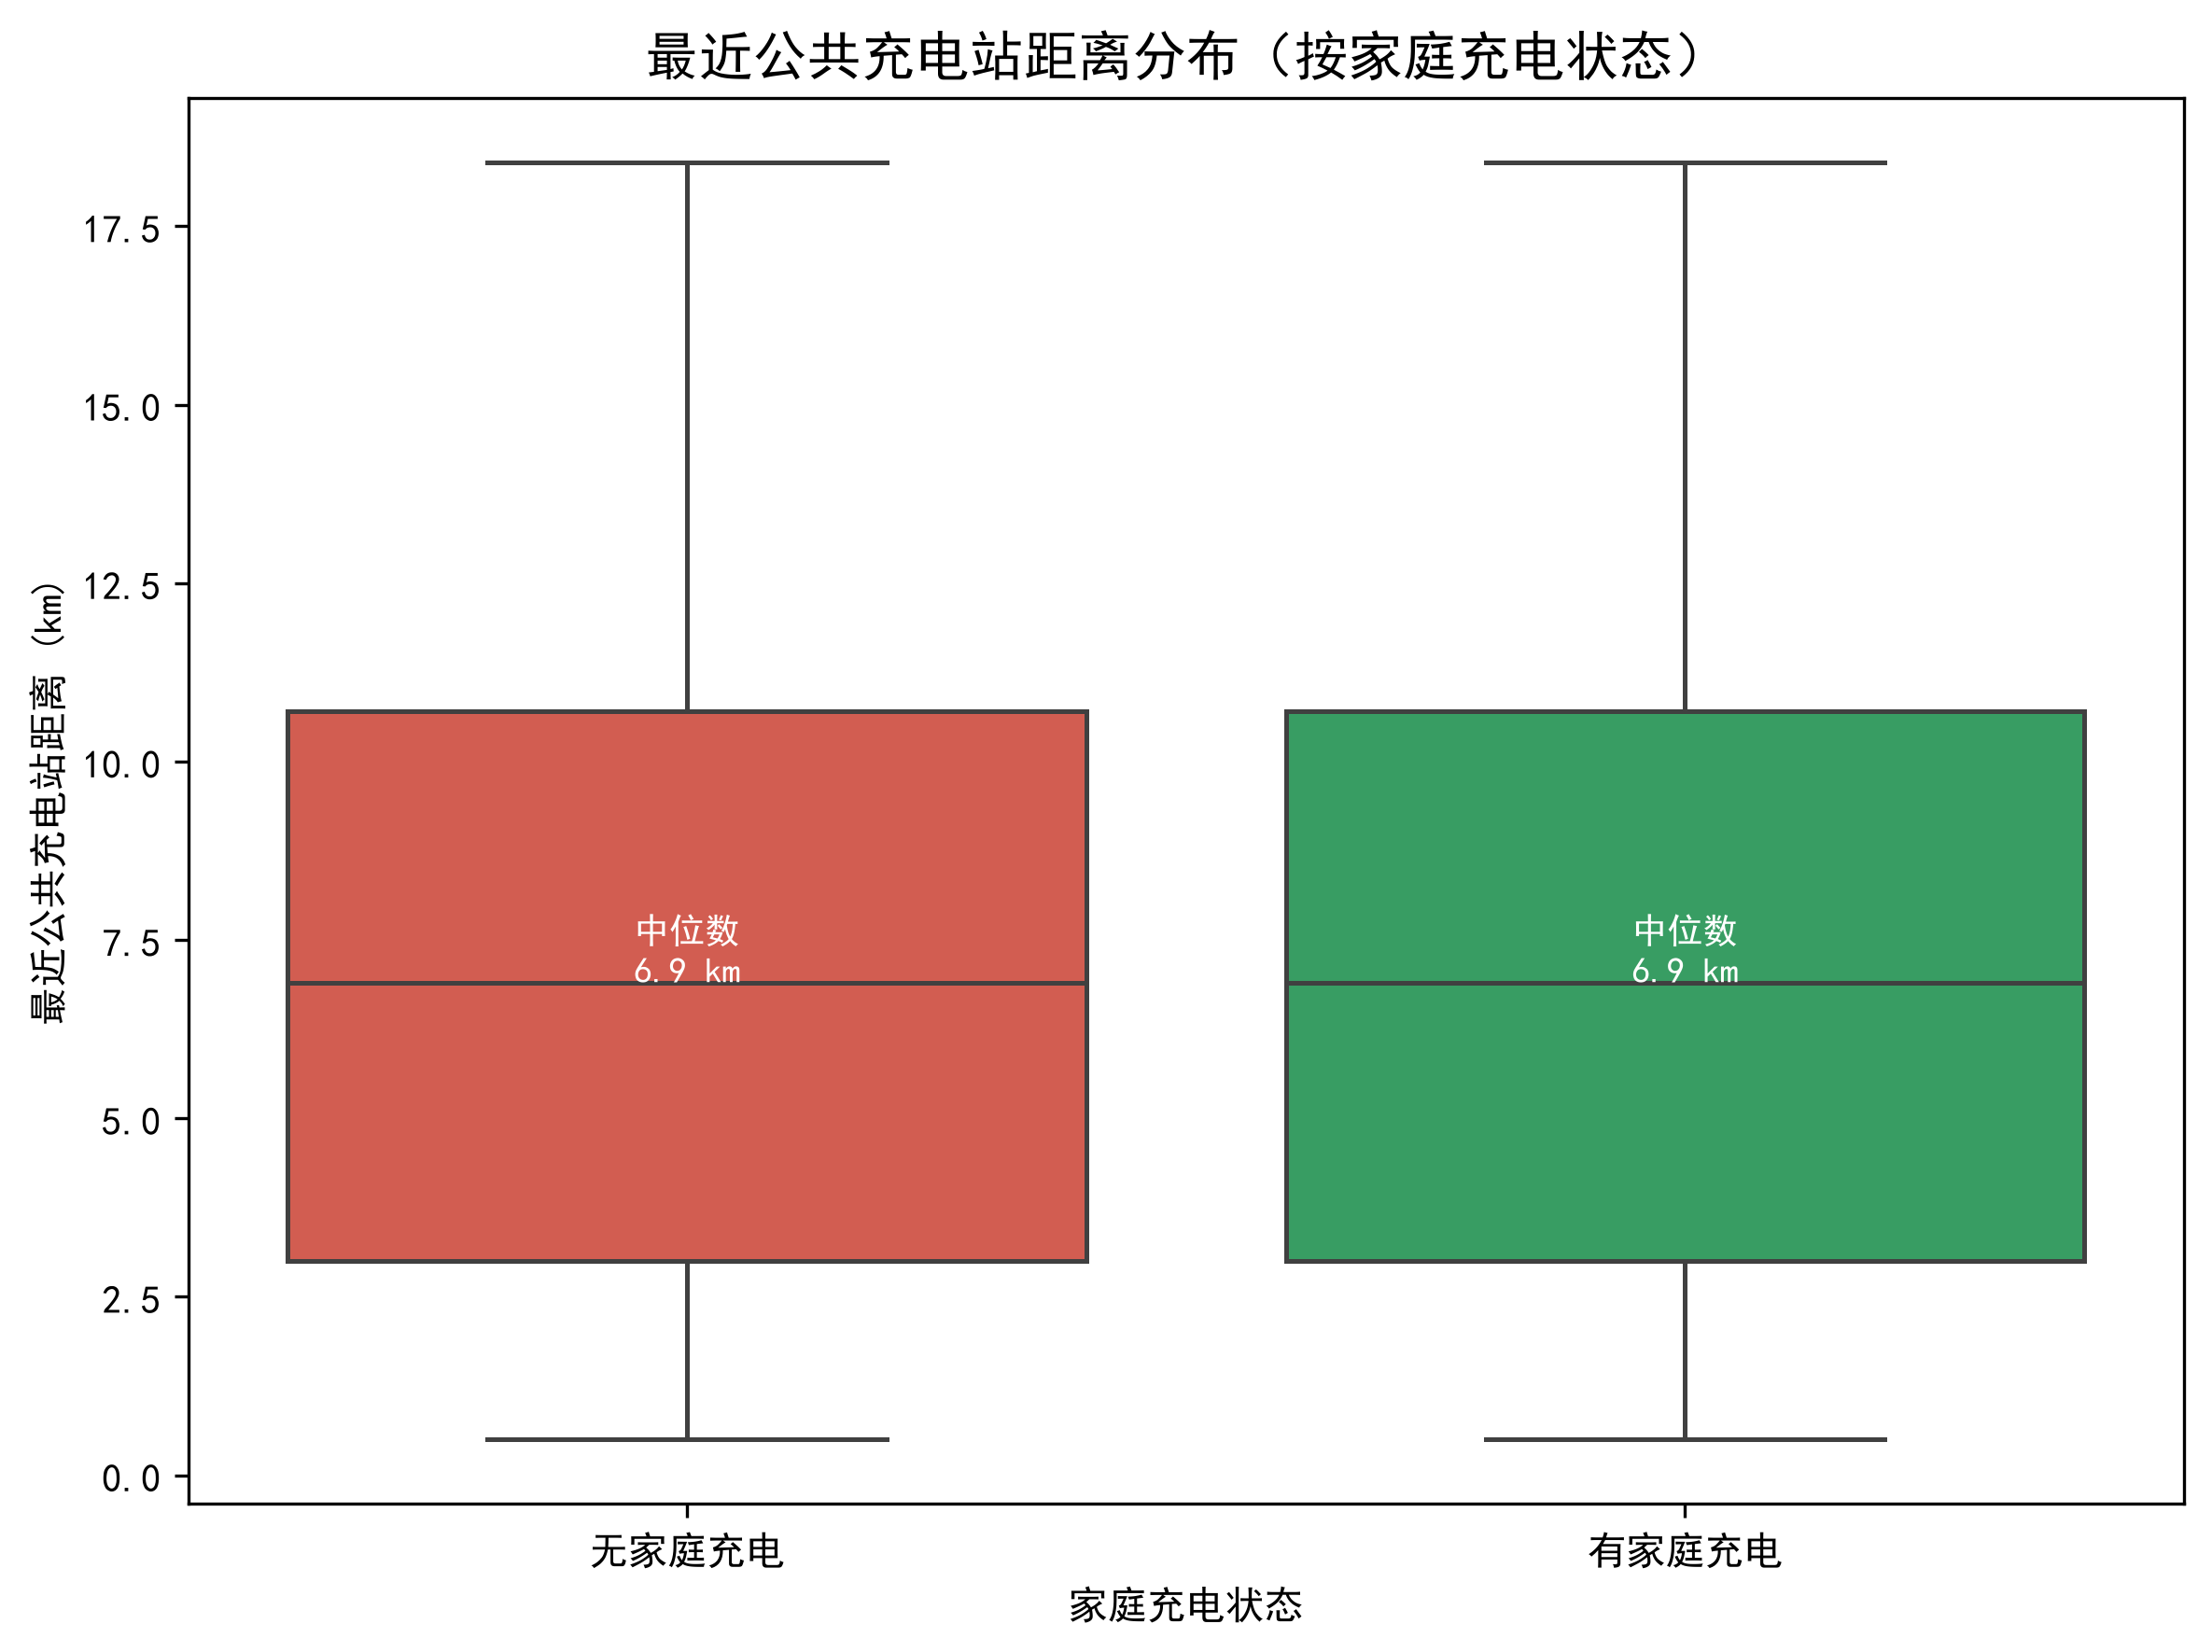
\includegraphics[width=0.7\textwidth]{figures/task2_charging_distance_boxplot.png}
\caption{最近充电站距离按家充状态分组箱线图}
\label{fig:t2_dist}
\end{figure}

\subsubsection{城市类型与家充状态}

三种城市类型的家充比例几乎完全一致（农村64.9\%，郊区65.2\%，城市64.8\%），差异不到0.4个百分点，如图\ref{fig:t2_city}所示。

\begin{figure}[H]
\centering
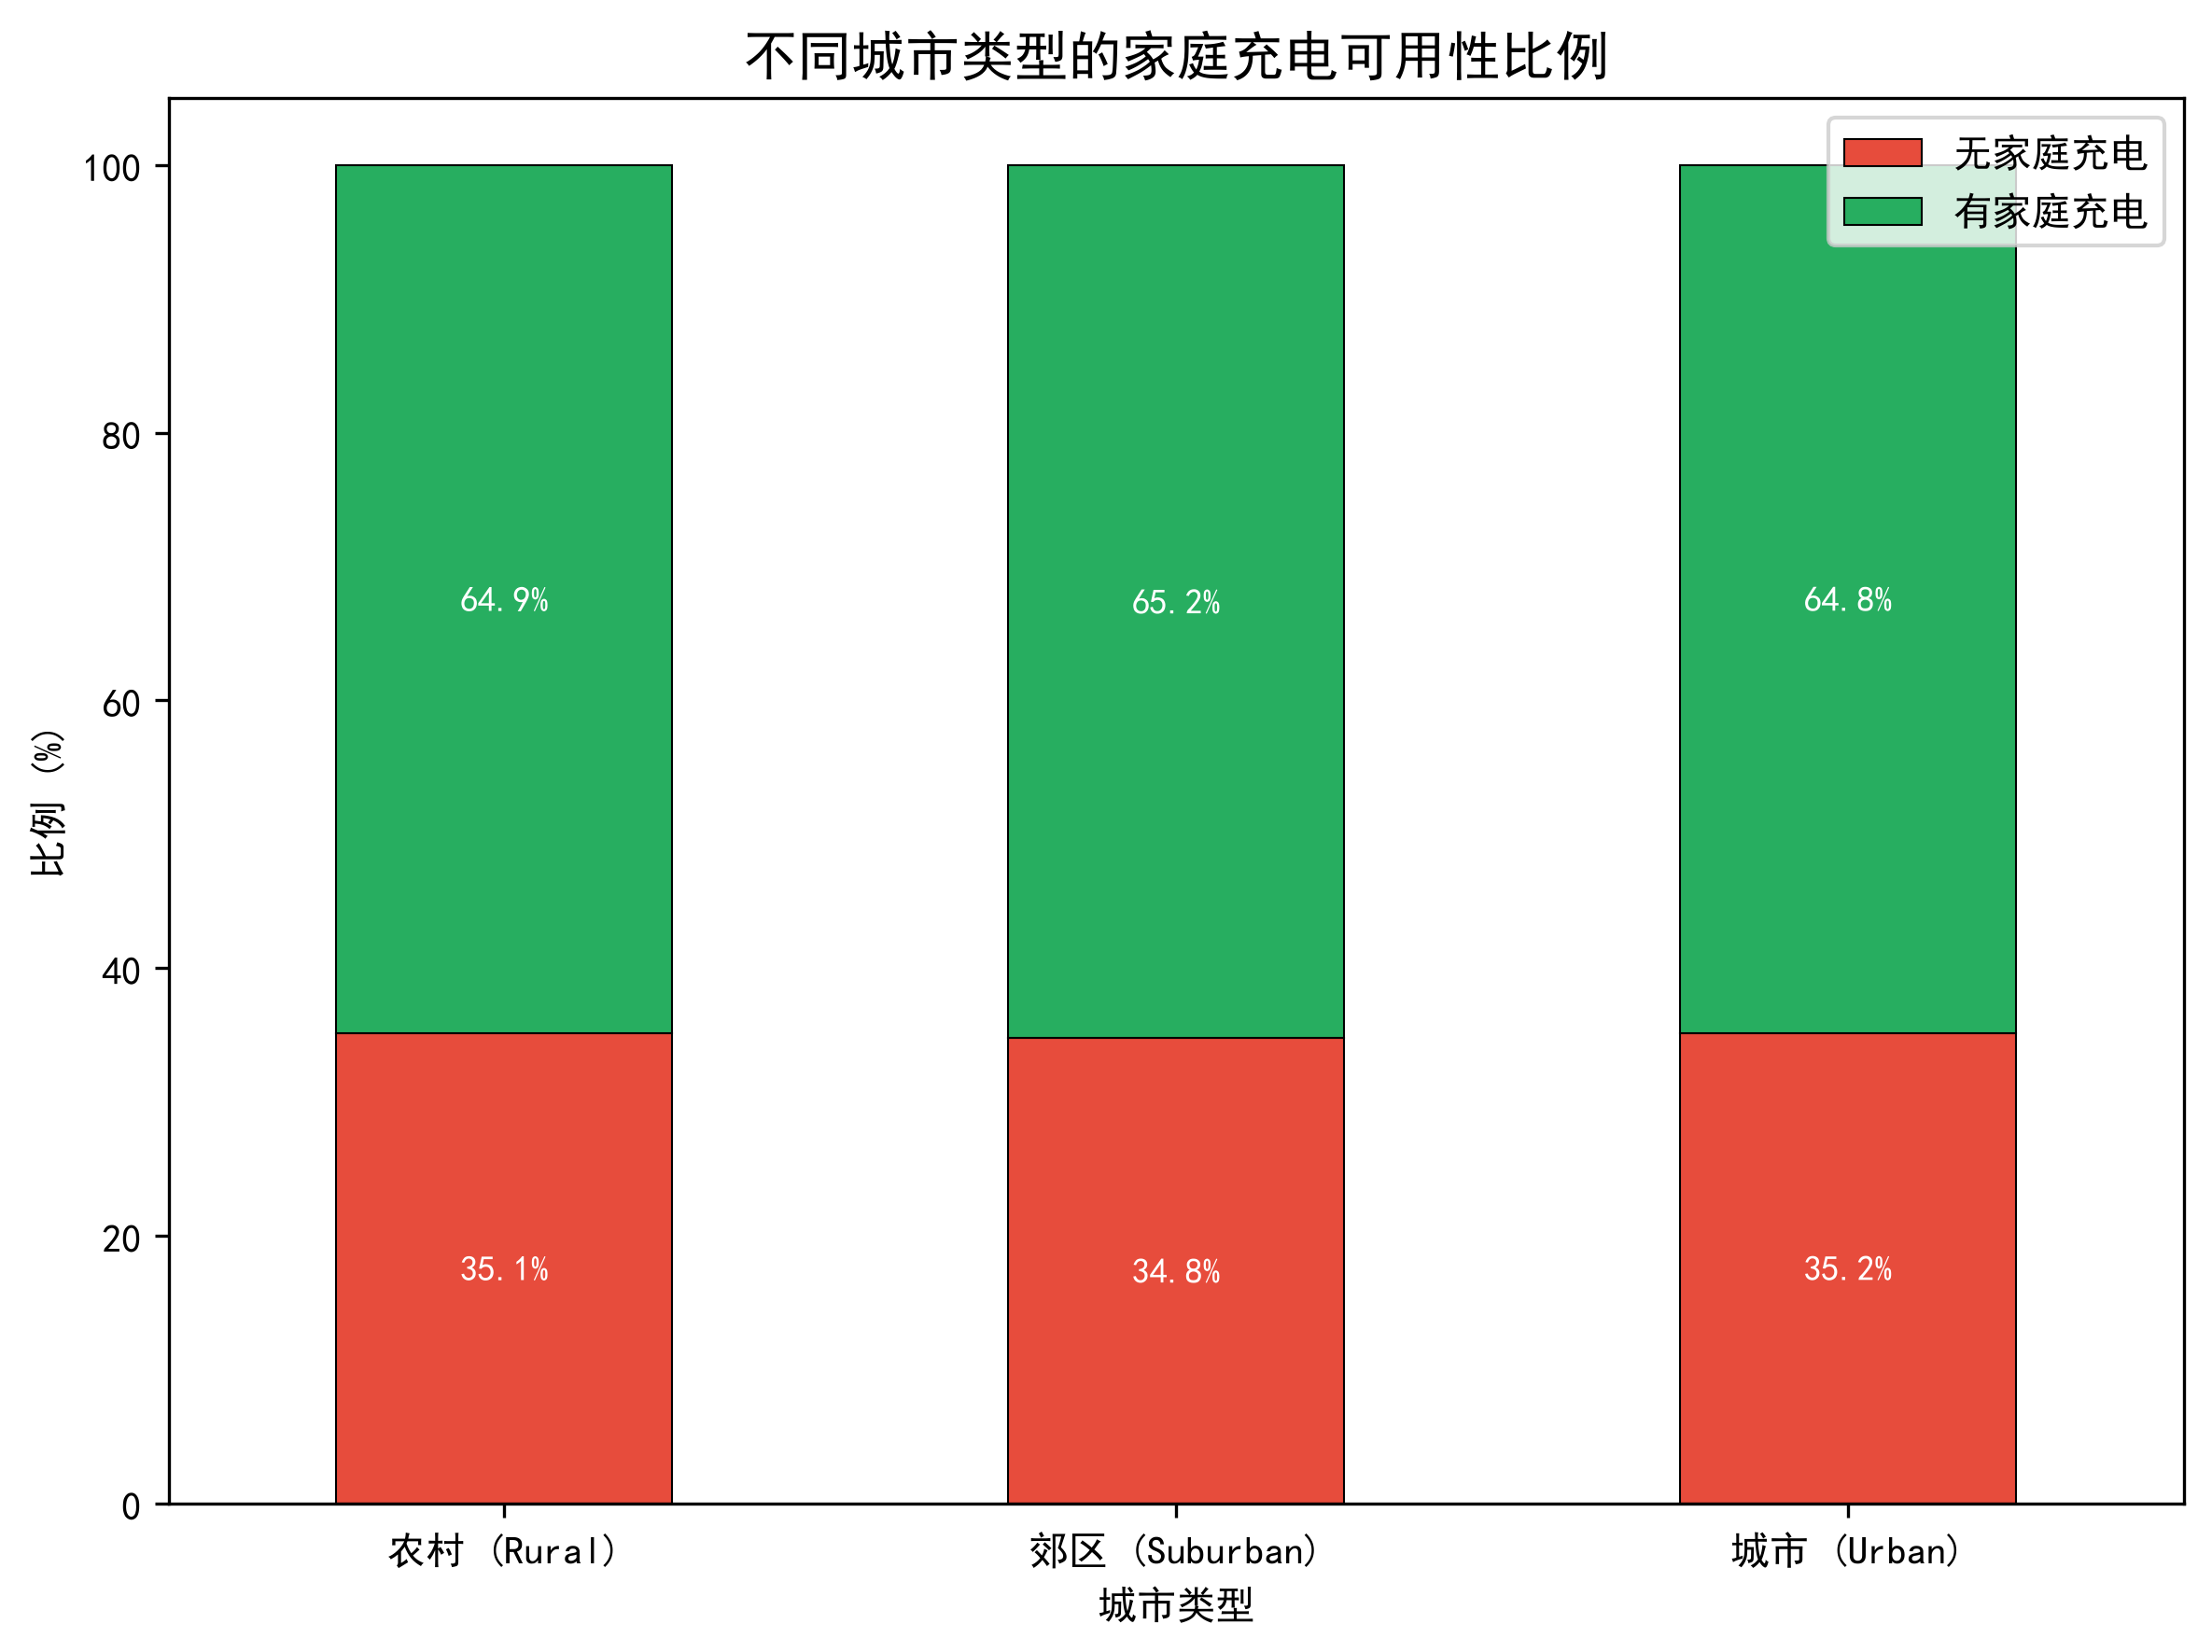
\includegraphics[width=0.75\textwidth]{figures/task2_citytype_stacked_bar.png}
\caption{不同城市类型的家庭充电可用性比例}
\label{fig:t2_city}
\end{figure}

城市类型在边际分布上对家充比例几乎无区分：农村64.9\%、郊区65.2\%、城市64.8\%。仅从比例数值判断，三类城市无差异。但这一事实不能简单理解为城市类型不相关——农村用户因公共充电设施匮乏更倾向于安装家用充电桩，城市用户可能出于环保意识与较高收入主动配备，郊区用户则受益于独立住宅提供的充裕安装空间。比例相等背后代表三种运行机制不同的驱动逻辑。同比例异成因的格局，为构造城市类型与其他变量的交互特征提供了依据。

\subsection{EDV预诊断：特征来源信号验证}

在进行超参数搜索之前，首先执行探索性数据验证（Exploratory Data Validation, EDV），以判定特征来源是否包含可供模型学习的有效信号。诊断结果见表\ref{tab:t2_edv}。

\begin{table}[H]
\centering
\caption{任务二EDV诊断结果}
\label{tab:t2_edv}
\begin{tabular}{lcc}
\toprule
\textbf{方案} & \textbf{验证ACC} & \textbf{ROC-AUC} \\
\midrule
多数类基线（全部预测为1） & 0.6498 & 0.5000 \\
严格特征 + Logistic Regression & 0.6498 & 0.4955 \\
严格特征 + ExtraTrees & 0.6485 & 0.4973 \\
严格特征 + HistGradientBoosting & 0.6498 & 0.4935 \\
严格特征 + CatBoost & 0.6498 & 0.4947 \\
加入真实采用意愿的诊断上界 + CatBoost & 0.6694 & 0.6160 \\
\bottomrule
\end{tabular}
\end{table}

排除ev\_adoption\_likelihood等下游变量后，全部可观测特征与家充标签的Pearson相关系数绝对值均在0.013以下。四种模型（逻辑回归、随机森林、直方梯度提升、CatBoost）的ROC-AUC值全部集中在0.50附近，准确率严格等于多数类基线。一项关键对照是：将真实采用意愿作为诊断上界加入特征集合后，准确率仅提升至0.6694，比基线高约2个百分点。该诊断信息在实际部署中无法获取，其意义在于为信号上限提供了定量参照。综合以上结果，特征来源本身缺乏有效信号是核心瓶颈，模型选择和调参策略并非限制因素。

\subsection{S0/S1/S2三方案对照设计}

基于EDV的诊断结论，设计了三套特征来源方案，逐层剥离瓶颈。

\textbf{S0：严格原始特征版（安全基线）}。仅使用city\_type、充电条件、经济与教育、车辆与出行需求等可观测特征，删除ev\_adoption\_likelihood、target\_ord、task3\_anxiety\_label在内的全部跨任务标签信息。S0是跨任务信息隔离的安全基线方案。

\textbf{S1：真实采用意愿上界版（诊断用途）}。在S0上加入真实ev\_adoption\_likelihood，仅用于回答一个问题："若采用意愿在预测时已知，最多能提升多少？"S1不作为可部署方案。

\textbf{S2：任务一OOF概率堆叠版（推荐主方案）}。不使用真实采用意愿标签，改为两步走：首先构建删除了home\_charging\_available字段的Task1-no-home模型，随后用该模型输出5个堆叠特征——stack\_p\_low/medium/high（三类别概率）、stack\_adoption\_expectation（期望值）与stack\_adoption\_entropy（预测熵）。堆叠概率在训练集内部通过5折交叉拟合生成（每折以其中4折训练Task1-no-home、预测剩余1折），验证集侧仅由全训练集模型做一次前向预测，从机制上杜绝标签泄漏。

\subsection{特征工程}

任务二共构造7个业务交互特征（表\ref{tab:t2_features}）。long\_commute\_flag与income\_quantile\_group的阈值分位数严格从训练集计算（fit=True），验证集则沿用训练集统计量（fit=False），杜绝信息从验证集回传至训练过程。

\begin{table}[H]
\centering
\caption{任务二业务交互特征}
\label{tab:t2_features}
\begin{tabular}{ccp{4cm}}
\toprule
\textbf{特征} & \textbf{计算方式} & \textbf{业务含义} \\
\midrule
charging\_scarcity & $\dfrac{\text{nearest\_station}}{\text{charge\_access} + 1}$ & 公共充电稀缺度 \\
long\_commute\_flag & $\mathbf{1}[\text{daily\_cm} > Q_{75}]$ & 长通勤标志 \\
income\_quantile\_group & 四分位数分4组 & 收入分位组 \\
vehicle\_renewal\_need & $\text{veh\_age} \times \text{fuel\_expense}$ & 车辆更新需求 \\
monthly\_travel\_intensity & $\text{weekly\_km} \times 4.33$ & 月行驶强度近似 \\
city\_charging\_interaction & $\text{city\_type} \times \text{nearest\_station}$ & 住宅环境交互（充电） \\
city\_income\_interaction & $\text{city\_type} \times \text{annual\_income}$ & 住宅环境交互（收入） \\
\bottomrule
\end{tabular}
\end{table}

\subsection{实验结果：负结果报告}

\subsubsection{S1诊断上界}

S1方案（加入真实ev\_adoption\_likelihood）的最高准确率为0.6694，仅超出多数类基线约2个百分点。这一数值构成了一个明确的结论：即使在预测时获得真实采用意愿信息，家充预测的准确率上限也十分有限。

\subsubsection{S2 OOF概率堆叠}

S2方案的结果如表\ref{tab:t2_results}所示。所有模型全部退化为多数类基线，ACC严格等于0.6498。

\begin{table}[H]
\centering
\caption{任务二S2方案验证集结果}
\label{tab:t2_results}
\begin{tabular}{lccc}
\toprule
\textbf{模型} & \textbf{ACC} & \textbf{ROC-AUC} & \textbf{说明} \\
\midrule
多数类基线 & 0.6498 & 0.5000 & 全预测为1 \\
LR (无权重) & 0.6498 & -- & 退化为多数类 \\
LR (balanced) & 0.4970 & -- & 随机猜测 \\
CatBoost 默认 & 0.6498 & 0.491 & 67次迭代即早停 \\
CatBoost CV最优 & 0.6498 & 0.489 & 3组参数全部同分 \\
\bottomrule
\end{tabular}
\end{table}

超参数搜索中3组候选参数在5折交叉验证下全部获得0.64975$\pm$0.00000的准确率，折间方差严格为零。零方差结果本身构成强诊断信号：最优阈值搜索仅需处理单一类别的概率分布，OOF概率几乎不随特征变化而波动。最优OOF阈值搜索结果为0.10（等价于几乎总是预测为1）。最终模型在验证集上3,502个无家充样本全部被误判为有家充，召回率等于零。

\subsection{原因分析与方法论贡献}

\subsubsection{不可观测因素分析}

家庭充电设施可用性主要由数据集中缺失的因素决定：

\begin{enumerate}[itemsep=0pt]
\item \textbf{住房属性}：是否拥有独立住宅或私人车库、房屋类型（公寓vs别墅）、房屋产权（自有vs租赁）；
\item \textbf{物业政策}：小区是否允许安装充电桩、是否有电力扩容条件；
\item \textbf{停车条件}：固定车位vs公共停车位。
\end{enumerate}

城市类型、收入、充电站距离等可观测变量与住房条件之间确实存在逻辑关联，然而这种关联在统计层面上过于间接，有监督学习模型无法从中提取有效信号。

\subsubsection{方法论贡献}

尽管预测结果不理想，整套研究流程在方法论层面提供了若干可复用的经验：

\begin{enumerate}[itemsep=0pt]
\item \textbf{EDV先行诊断框架}：在部署大规模超参数搜索之前，先通过多模型对比快速判断特征来源是否包含可学习信号，避免在无效数据上投入过度的优化资源；
\item \textbf{S0/S1/S2消融体系}：以严格特征、诊断上界、跨任务堆叠三层级对照设计，逐一排除模型选择、调参不足、特征工程缺失等可能的失败原因；
\item \textbf{跨任务无泄漏堆叠设计}：Task1-no-home模型删除home\_charging\_available字段后再生成OOF概率，两阶段推理链可完整复现且保证信息隔离；
\item \textbf{负结果的诚实报告}：从EDV诊断至逐层消融至最终判定的完整链路，可作为同类问题中信号验证与瓶颈定位的复用模板。
\end{enumerate}
